\chapter{Deep reinforcement learning}


Deep learning has a large impact on neuroscience. For instance:
\begin{casestudy}[Neural network to represent parietal neurons \cite{parietal_network}]
    A monkey is tasked to maintain fixation at a point with a stimulus visible within its receptive field. The fixation point and the stimulus are moved together so that, for the retina, the stimulus is at the same retinal coordinate.

    \begin{figure}[H]
        \centering
        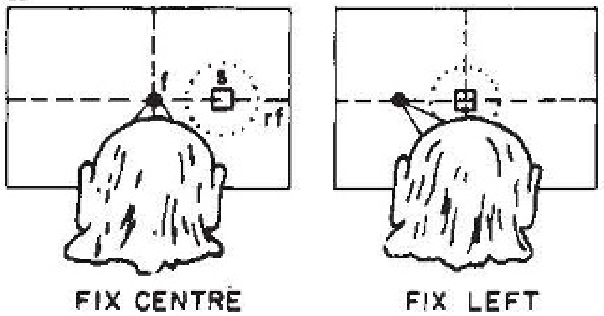
\includegraphics[width=0.3\linewidth]{./img/monkey_parietal1.png}
    \end{figure}

    In the parietal cortex, the firing of neurons depends on:
    \begin{itemize}
        \item The position of the stimulus in the receptive field.
        \item The position of the eyes in the orbit.
    \end{itemize}

    \begin{figure}[H]
        \centering
        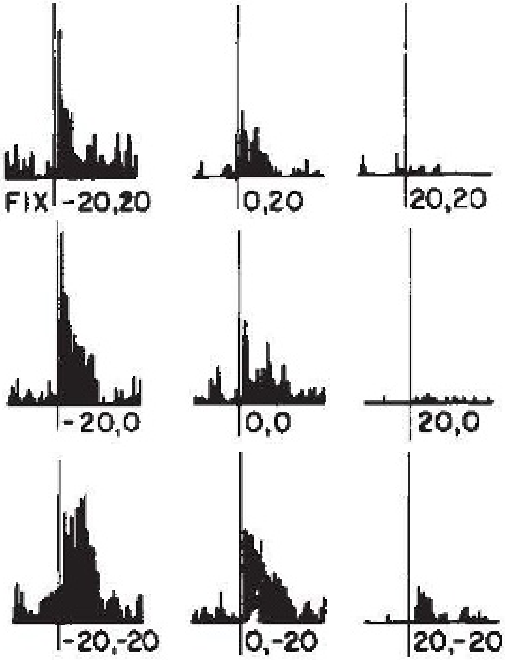
\includegraphics[width=0.2\linewidth]{./img/monkey_parietal2.png}
        \caption{Readings of a parietal neuron at different fixation points}
    \end{figure}

    Using the parietal readings, the authors were able to create a network to predict the spatial position of objects.
    
    \indenttbox
    \begin{remark}
        This is one of the first successful applications of neural networks in neuroscience.
    \end{remark}
\end{casestudy}


\section{Deep reinforcement learning applications}

\begin{description}
    \item[Reinforcement learning] \marginnote{Reinforcement learning}
        Given a state and a set of stimuli, find the best policy to maximize future reward.
        
        \begin{remark}
            Differently from supervised learning, in reinforcement learning:
            \begin{itemize}
                \item The agent does not know the correctness of its actions.
                \item The agent has to learn the best policy in the distribution of policies. 
                    In contrast, in supervised learning the model needs to learn to generalize different distributions (e.g. different images of the same class).
            \end{itemize}
        \end{remark}

        \begin{remark}
            In early RL work, a tabular state representation was adopted. 
            This approach was unable to generalize as it was not possible to distinguish similar states. 
            A workaround is to use function approximations to encode states into a feature space.
        \end{remark}

    \item[Deep reinforcement learning] \marginnote{Deep reinforcement learning}
        Use a neural network to learn the representation of the environment and the policy solving an RL problem.

        \begin{casestudy}[TD-Gammon \cite{td_gammon}]
            TD-Gammon is a neural network trained using a form of temporal difference learning to play the game of backgammon.
            Due to instability, the results were not satisfying.
        \end{casestudy}

        \begin{casestudy}[Atari deep Q-learning \cite{atari_qlearning, qlearning_frostbite}]
            It has been shown that deep Q-learning networks (DQN) can successfully learn to play classic Atari games at human-level performance.
            However, the learning method is significantly different from human's:
            \begin{itemize}
                \item Professional gamers are able to reach good scores in approximately $2$ hours.
                \item DQN requires 200 million frames ($\sim 942$ hours) with experience replay where each frame is replayed approximately eight times during learning.
            \end{itemize}

            Comparison with different variants of DQN shows that agents require more time to reach human-like performance but are also able to outperform them given enough time.
            \begin{figure}[H]
                \centering
                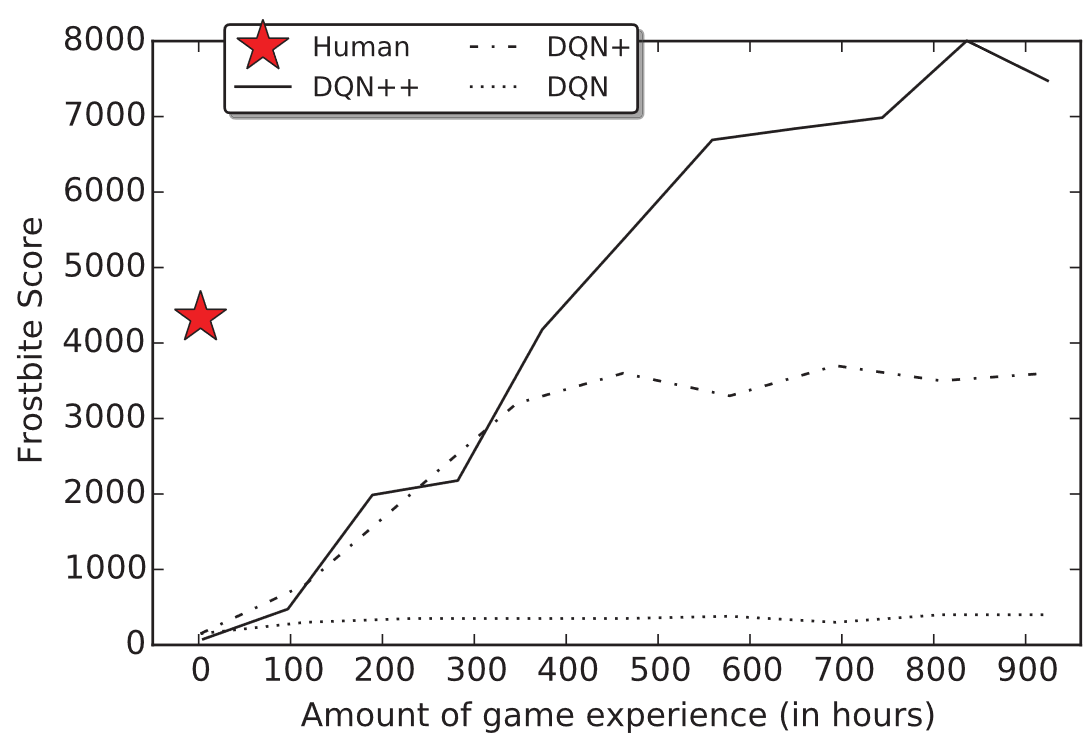
\includegraphics[width=0.4\linewidth]{./img/atari_dqn1.png}
                \caption{Comparison on the Frostbite game}
            \end{figure}
        \end{casestudy}

        \begin{remark}
            Speculations on possible ways to improve artificial agents are:
            \begin{itemize}
                \item Provide causal models of the world to support explanation and understanding (at this stage, agents are similar to humans with neural lesions that make them unable to understand causal relationships).
                \item Ground learning on intuitive theories of physics and psychology.
                \item Learn how to learn.
            \end{itemize}
        \end{remark}
\end{description}


\subsection{Inefficiency factors}

There are at least two factors that cause the sample inefficiency of deep reinforcement learning networks.
\begin{description}
    \item[Slow parameter adjustments] \marginnote{Slow parameter adjustments}
        Parameters of a neural network are updated by small steps as larger steps might cause the problem of "catastrophic interference".

    \item[Bias-variance tradeoff] \marginnote{Bias-variance tradeoff}
        Neural network have a weak inductive bias:
        \begin{itemize}
            \item A learning procedure with a weak inductive bias (and large variance) is able to learn a wide range of patterns but is generally less sample-efficient.
            \item A learning procedure with a strong inductive bias can use its prior hypotheses to rapidly solve the task, provided that the hypotheses are suited for that specific task.
        \end{itemize}
\end{description}


\section{Episodic reinforcement learning}

\begin{description}
    \item[Episodic RL] \marginnote{Episodic RL}
        Non-parametric (examplar-based) RL approach that learns from past experience.

        The agent explicitly records past events that are used for future decision-making.

        \begin{remark}
            This can be seen as a third action selection method together with model-based and model-free approaches.
        \end{remark}

    \item[Long-term memory] \marginnote{Long-term memory}
        Inactive past memories that have to be reactivated to use them. In humans, it comes in different forms:
        \begin{descriptionlist}
            \item[Declarative/Explicit]
                Memory that can be expressed in a propositional form (i.e. by words).
                \begin{description}
                    \item[Episodic] 
                        Memory related to a specific experience in space and time.

                    \item[Semantic] 
                        Memory related to the shared aspects of many episodic memories (can be seen as an average).
                \end{description}

            \item[Procedural/Implicit] 
                Memory involving practical procedures (knowing-how). It can be related to model-free approaches.
        \end{descriptionlist}

        \begin{figure}[H]
            \centering
            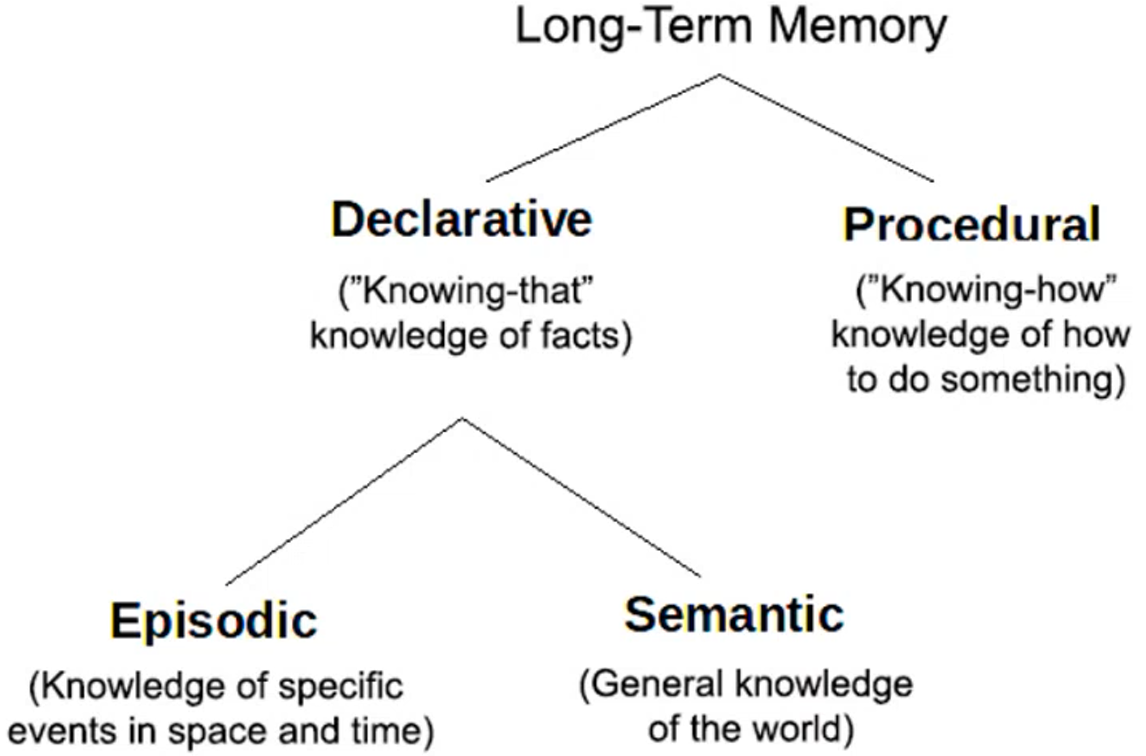
\includegraphics[width=0.35\linewidth]{./img/long_term_memory.png}
        \end{figure}

        \begin{remark}
            On the other spectrum, there are short-term and working memories.
            The former, once formed, is sort of read-only (e.g. repeat a sequence of numbers). The latter allows the manipulation of its content (e.g. repeat a sequence of numbers in reverse order).
        \end{remark}

    \item[Complementary learning systems (CLS) theory] \marginnote{Complementary learning systems (CLS) theory}
        Theory stating that intelligent agents possess two learning systems involving two parts of the brain:
        \begin{descriptionlist}
            \item[Neocortex] 
                Slowly acquires structured knowledge of the environment that is shaped based on the structure of past experience.
            \item[Hippocampus] 
                Allows to rapidly learn spatial and non-spatial features of a particular experience (episodic memory).
                It forms the initial memory of an episode and interacts with the cortex by replaying it multiple times to eventually form a lasting memory (reinstatement).
                \begin{remark}
                    Patients without the hippocampus cannot remember events that happened close in time.
                \end{remark}
        \end{descriptionlist}
        \begin{figure}[H]
            \centering
            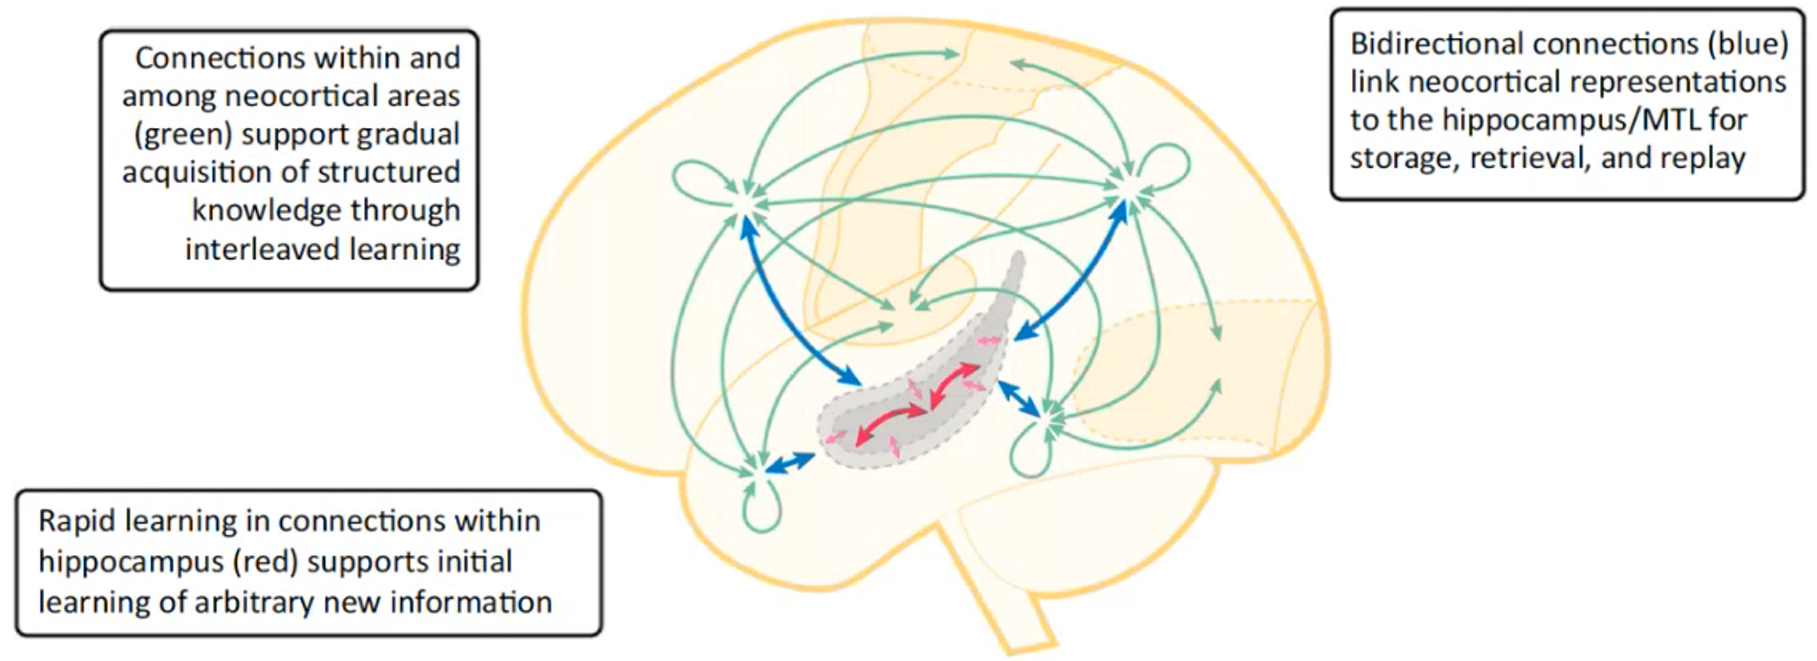
\includegraphics[width=0.7\linewidth]{./img/cls_theory.png}
            \caption{Pathways of the CLS theory}
        \end{figure}

        \begin{casestudy}[Neural episodic control \cite{nec}]
            In neural episodic control (NEC), an agent stores each encountered state with the discounted sum of rewards of $n$ future steps to form an episodic memory associated with the state and the received reward.

            NEC consists of three components:
            \begin{itemize}
                \item A convolutional network to process the image at state $s$ and convert it into a key to query the memory,
                \item A set of memory modules (differentiable neural dictionary),
                \item A final network that converts action memories into $Q(s, a)$ values.
            \end{itemize}
            To estimate the value of a state, the agent computes the sum of the stored discounted rewards weighted depending on the similarity between the stored states and the new state.

            \begin{figure}[H]
                \centering
                \begin{subfigure}{0.56\linewidth}
                    \centering
                    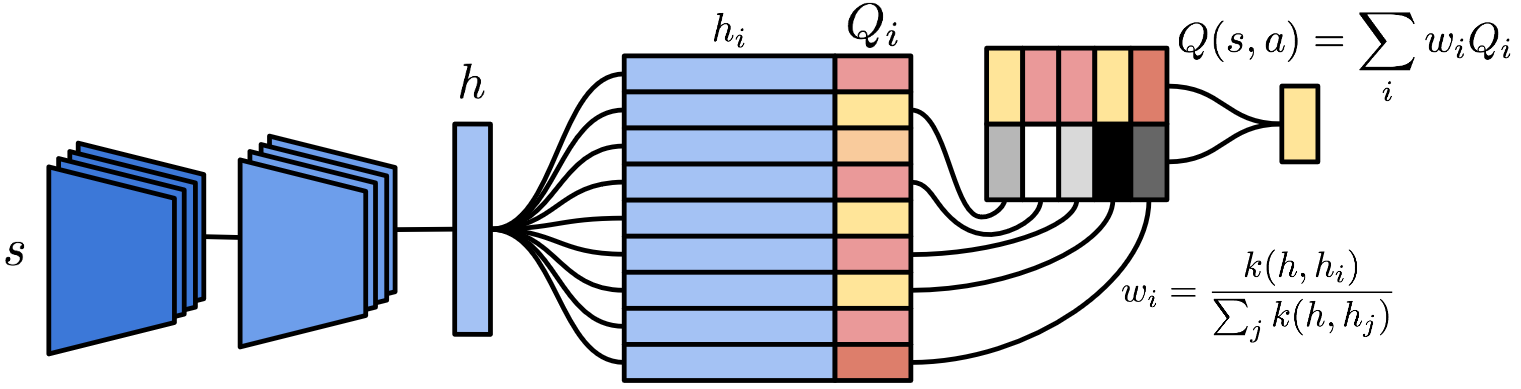
\includegraphics[width=0.95\linewidth]{./img/nec1.png}
                    \caption{NEC structure}
                \end{subfigure}
                \begin{subfigure}{0.42\linewidth}
                    \centering
                    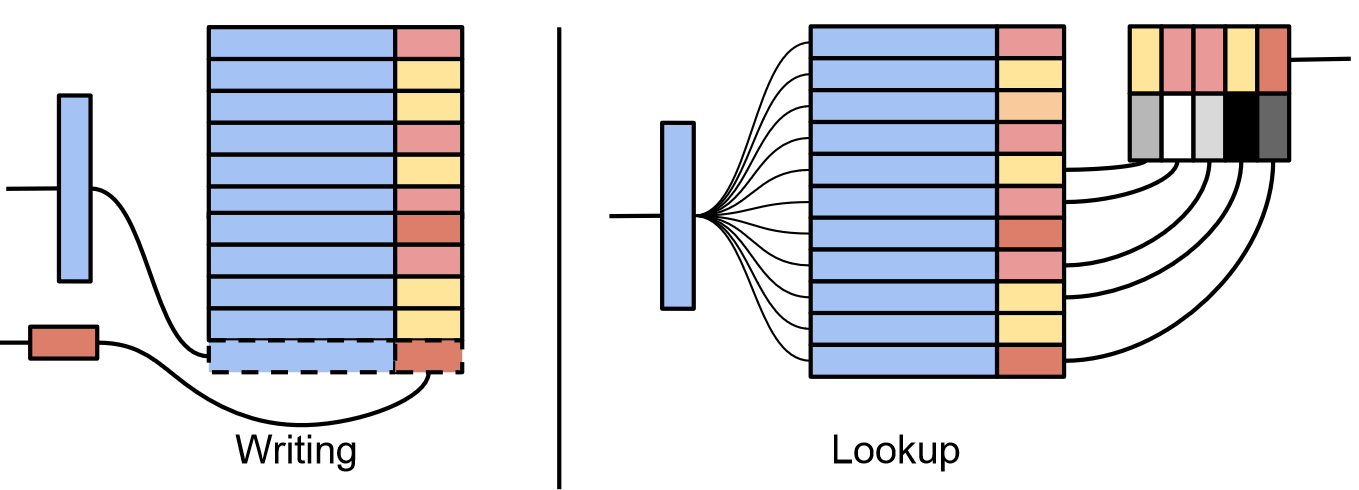
\includegraphics[width=0.95\linewidth]{./img/nec2.png}
                    \caption{Possible memory operations}
                \end{subfigure}
            \end{figure}

            This allows to make the system faster and more efficient.
            \begin{figure}[H]
                \centering
                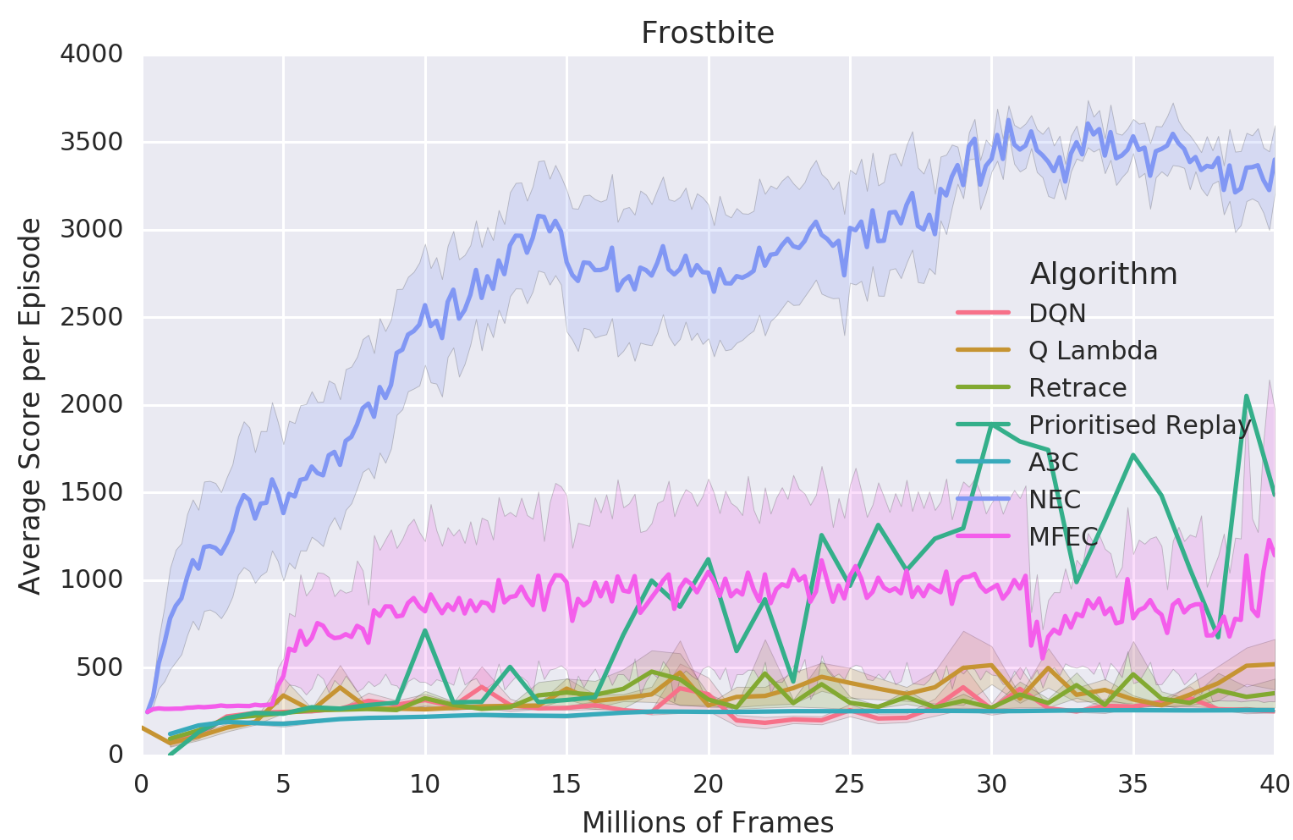
\includegraphics[width=0.5\linewidth]{./img/nec3.png}
                \caption{Results on Frostbite}
            \end{figure}
        \end{casestudy}

        \begin{remark}
            The difference between model-free and episodic RL is how they store experiences:
            \begin{itemize}
                \item In model-free RL, each individual experience is integrated into a cached value and stored in memory. The cached value is used to make decisions.
                \item In episodic RL, each individual experience and its reward is stored in memory. Each episodic trace is weighted depending on the similarity to the current state to make a decision.
            \end{itemize}

            \begin{figure}[H]
                \centering
                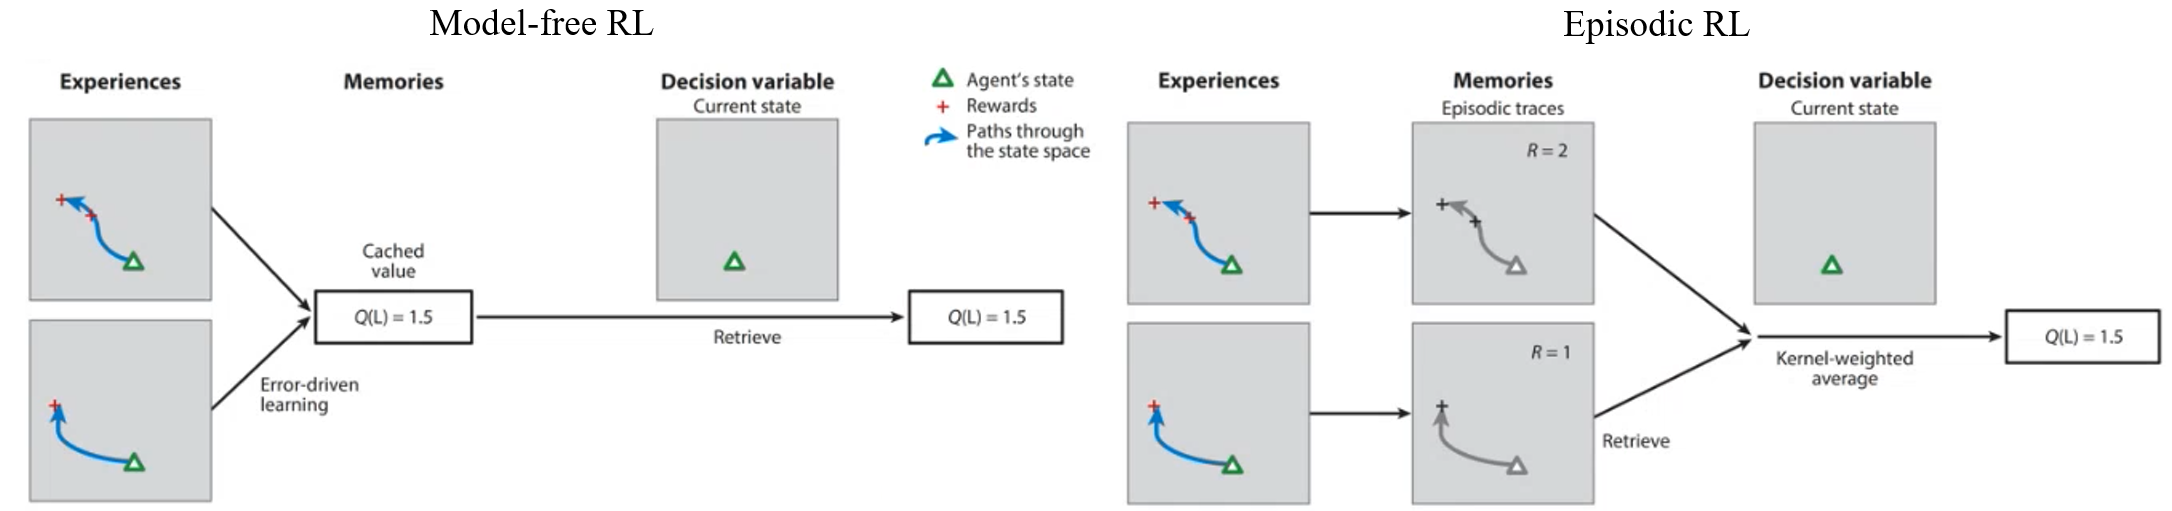
\includegraphics[width=0.9\linewidth]{./img/model_free_vs_episodic.png}
            \end{figure}
        \end{remark}

        \begin{remark}
            Episodic control and replay are not the same thing.
        \end{remark}

        \begin{casestudy}[Replay in rats]
            The movements and the activity of a neuron (place cell) in the hippocampus of a rat are recorded.
            It has been observed that the place cell fires only at a specific spatial area (and it changes if the rat is moved to another environment).
            \begin{figure}[H]
                \centering
                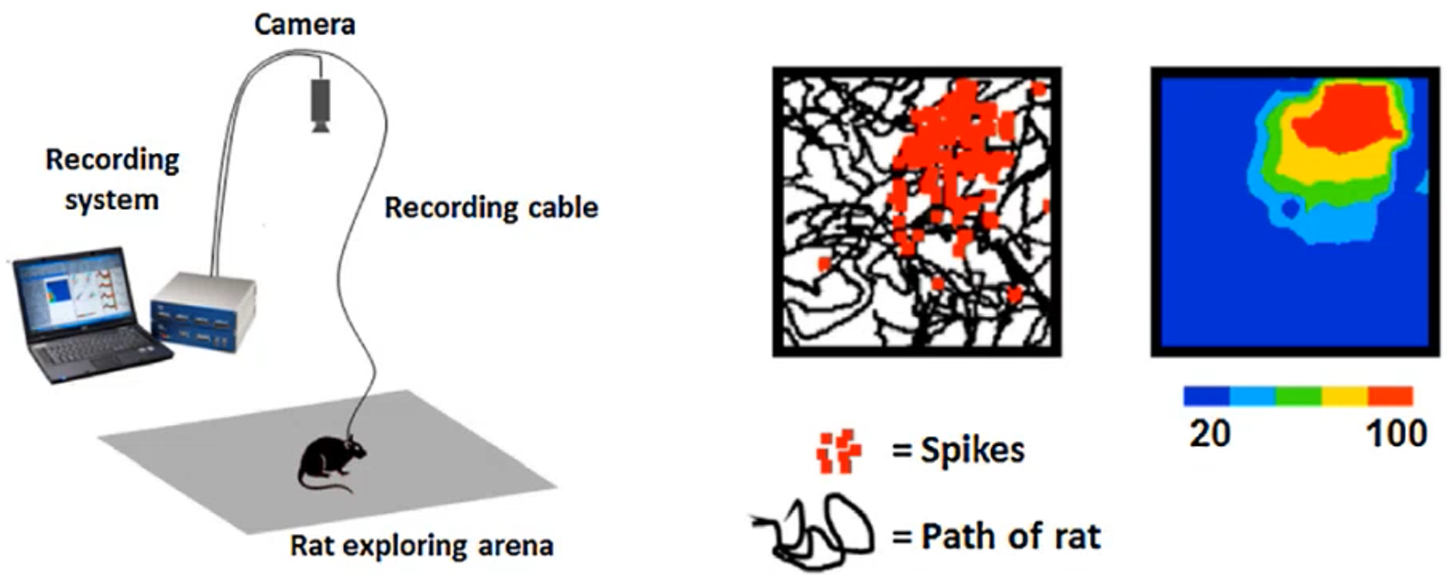
\includegraphics[width=0.55\linewidth]{./img/hippocampus_replay1.png}
            \end{figure}

            \indenttbox
            \begin{remark}
                Grid cells are another type of cells in the medial entorhinal cortex that fire based on spatial features.
                Differently from place cells, this type of cell is active in multiple zones arranged in a regular manner (i.e. triangular or hexagonal units).

                In other words, place cells are based on landmarks and grid cells are based on self-motion.
                \begin{figure}[H]
                    \centering
                    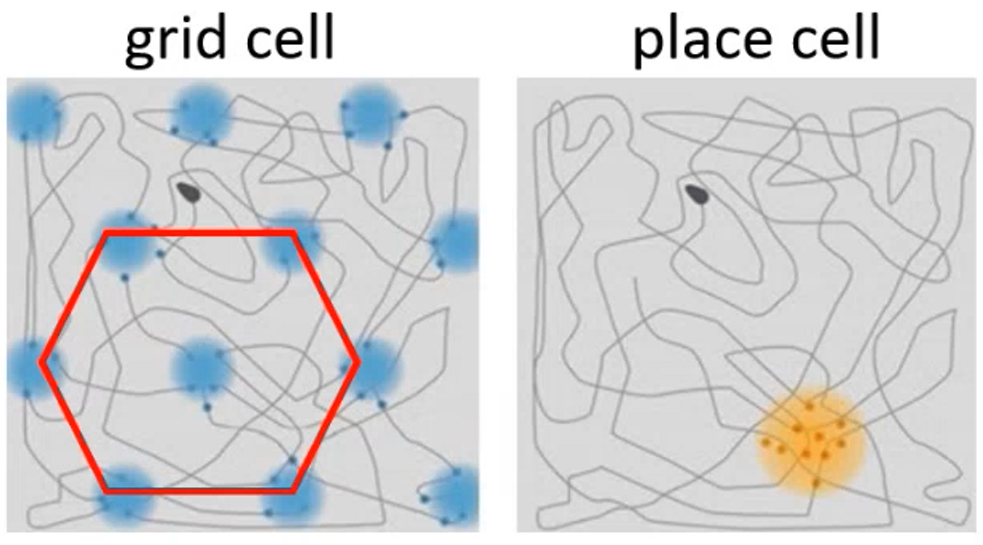
\includegraphics[width=0.25\linewidth]{./img/grid_place_cell.png}
                \end{figure}
            \end{remark}

            By placing the rat on a triangular track where some reward is available, a correlation between two place cells have been recorded.
            \begin{figure}[H]
                \centering
                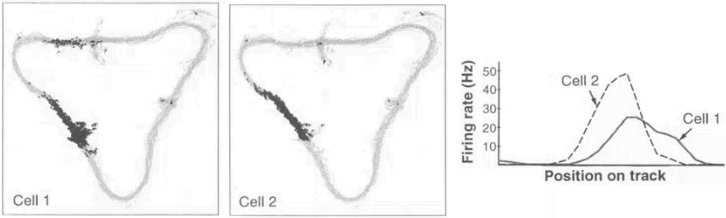
\includegraphics[width=0.6\linewidth]{./img/hippocampus_replay2.png}
            \end{figure}

            It has been observed that the rat replays the episode as the activation of the two cells becomes correlated also when asleep.
            \begin{figure}[H]
                \centering
                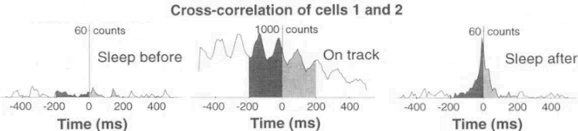
\includegraphics[width=0.6\linewidth]{./img/hippocampus_replay3.png}
            \end{figure}
        \end{casestudy}

        \begin{casestudy}[Memory in human decisions \cite{memory_decision}]
            \phantom{}
            \begin{description}
                \item[Experiment 1] 
                    In each trial, candidates are asked to choose a slot machine to spin (bandit problem). Each slot has a different point reward that changes at each trial.
                    \begin{figure}[H]
                        \centering
                        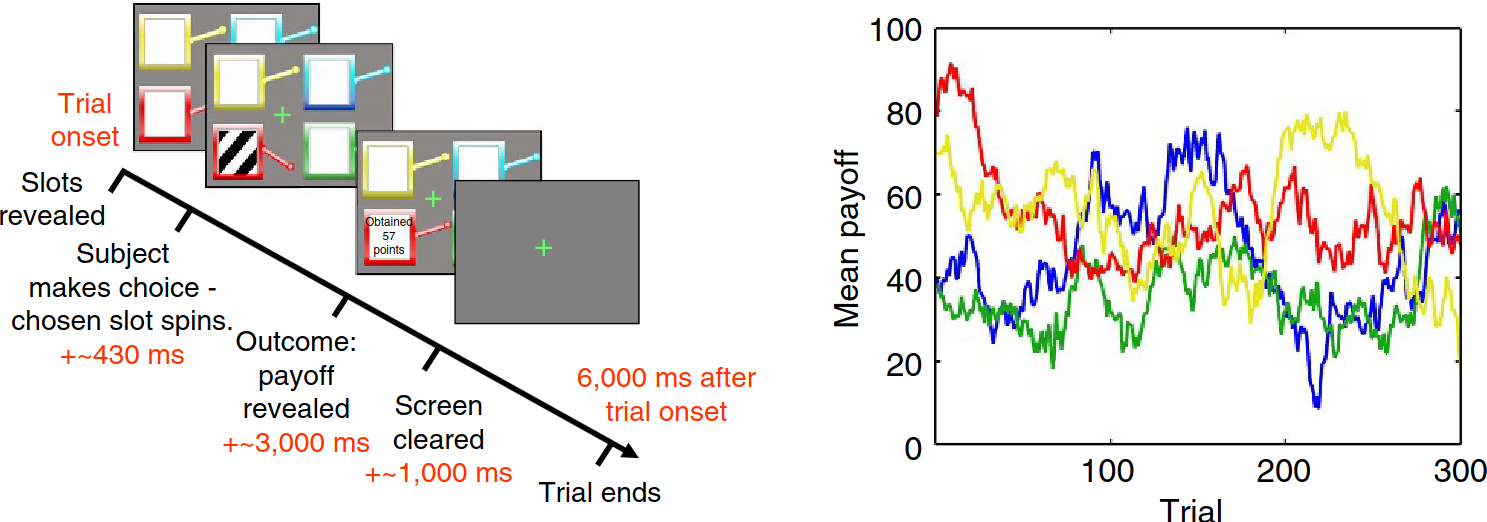
\includegraphics[width=0.55\linewidth]{./img/memory_decision1.png}
                    \end{figure}
        
                    Two models are used to attempt to fit the behavior of humans:
                    \begin{enumerate}
                        \item A temporal difference learning approach with a running average estimate of action value.
                        \item A model that samples from previous experiences to estimate action value. More recent experiences are more likely to be sampled.
                    \end{enumerate}
                    It has been observed that each subject is more similar to a sampling model.

                \item[Experiment 2]
                    In the previous experiment, it was not possible to determine which individual trial a participant sampled to make a decision.

                    The experiment is therefore simplified with two slots with two possible outcomes ($\pm 5$ dollars) and in some of the trials (32) the choice is also paired with a probe image whose purpose is to bring to mind that specific trial.

                    After the first round of trials, candidates are asked to perform a second round. Now, before making a choice, one of the probe images is shown to the candidate.
                    
                    Results show that, by showing the image, decisions are more biased favoring the winning slot and avoiding the losing slot.

                    \begin{figure}[H]
                        \centering
                        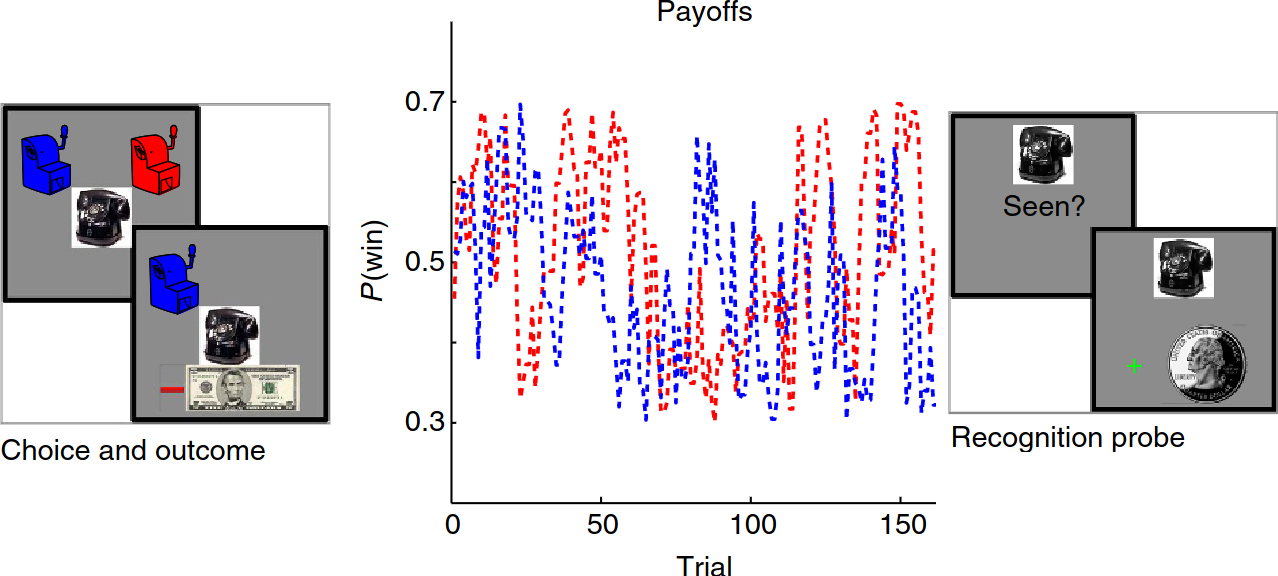
\includegraphics[width=0.6\linewidth]{./img/memory_decision2.png}
                    \end{figure}
            \end{description}
        \end{casestudy}
\end{description}



\section{Meta-learning}

\begin{description}
    \item[Meta-learning] \marginnote{Meta-learning}
        Use past experience to speed up new learning.

        \begin{remark}
            Animals use meta-learning as learning does not happen from scratch.
        \end{remark}
\end{description}

\begin{casestudy}[Meta-learning in monkeys \cite{monkey_meta_learning}]
    Monkeys are presented with two unfamiliar objects and are asked to grab one of them.
    Under an object lays either food or nothing.
    The same procedure is repeated for six trials and the position of the two objects can be swapped.
    After the round of trials, new rounds are repeated with new objects.

    It has been observed that after some rounds, monkeys are able to learn the task in one shot.

    \begin{figure}[H]
        \centering
        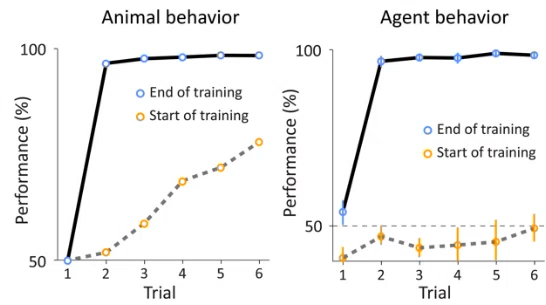
\includegraphics[width=0.4\linewidth]{./img/monkey_meta1.png}
        \caption{Monkeys (left) and machine simulated (right) results}
    \end{figure}
\end{casestudy}

\begin{remark}
    Learning is nested at multiple scales:\\[0.5em]
    \begin{minipage}{0.55\linewidth}
        \begin{itemize}
            \item At the highest level, learning involves evolution and aims to learn highly invariant universal structures (e.g. intuitive physics).
            \item At the middle level, learning involves the general structure of different tasks (e.g. how to play video games).
            \item At the innermost level, learning involves a fast adaptation to specific tasks (e.g. how to play a new video game).
        \end{itemize}
    \end{minipage}
    \begin{minipage}{0.4\linewidth}
        \centering
        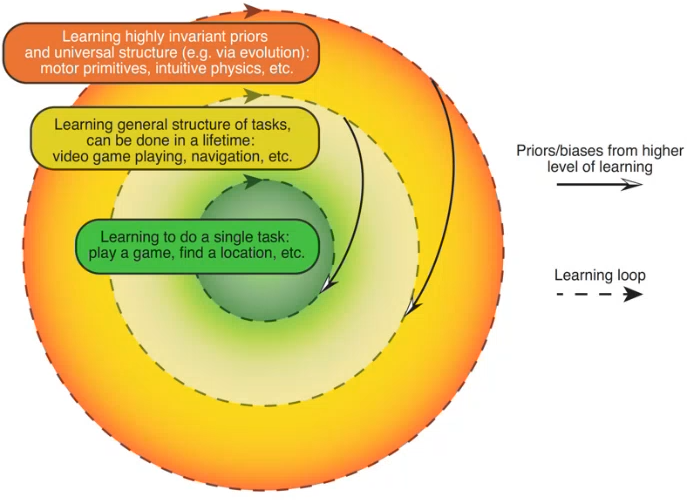
\includegraphics[width=0.95\linewidth]{./img/nested_learning.png}
    \end{minipage}
\end{remark}

\begin{casestudy}[Meta-learning RNN model \cite{human_meta_learning}]
    Meta-learning can be modeled using an RNN that is used to solve a task.
    At each step, the network takes, apart from the input, the correct output of the previous step that can be seen as a form of supervision.

    \begin{figure}[H]
        \centering
        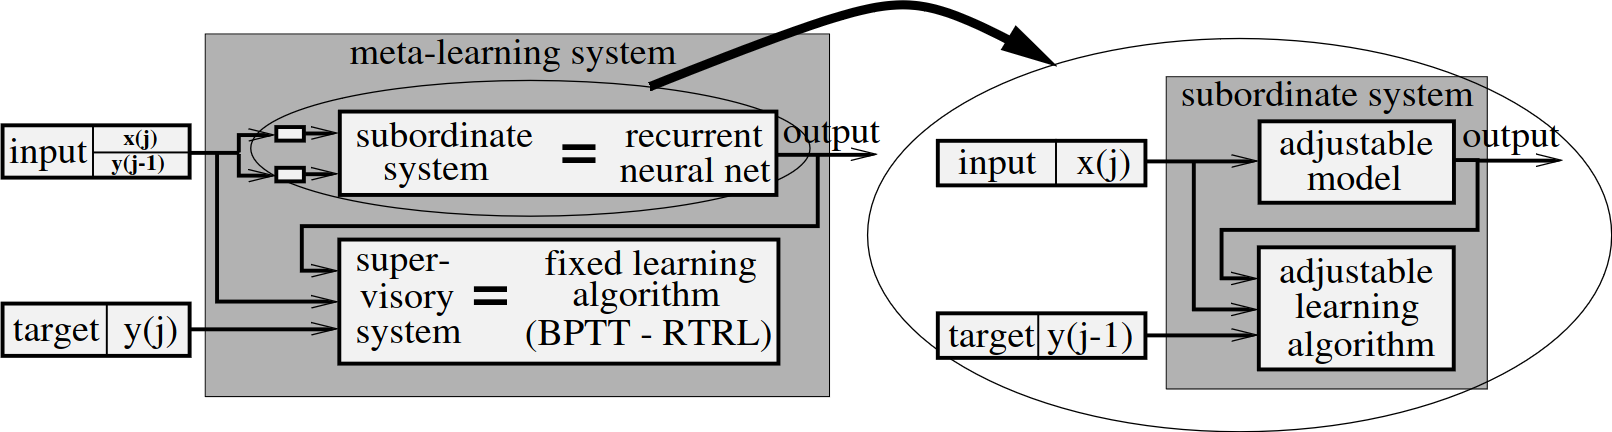
\includegraphics[width=0.6\linewidth]{./img/human_meta.png}
    \end{figure}
\end{casestudy}

\begin{description}
    \item[Meta-reinforcement learning] \marginnote{Meta-reinforcement learning}
        Learning system that adjusts another learning system.
        It can be described with two loops:
        \begin{descriptionlist}
            \item[Outer-loop] 
                System that uses its experience over many task contexts to adjust the parameters of the inner-loop.
                It is a slow system as it learns multiple tasks.
            \item[Inner-loop] 
                System that is tuned by the outer-loop.
                It is a fast system that needs to adapt to a specific task.
                \begin{example}
                    An RNN that tasks as input the last action, reward and state.
                \end{example}
        \end{descriptionlist}
        \begin{figure}[H]
            \centering
            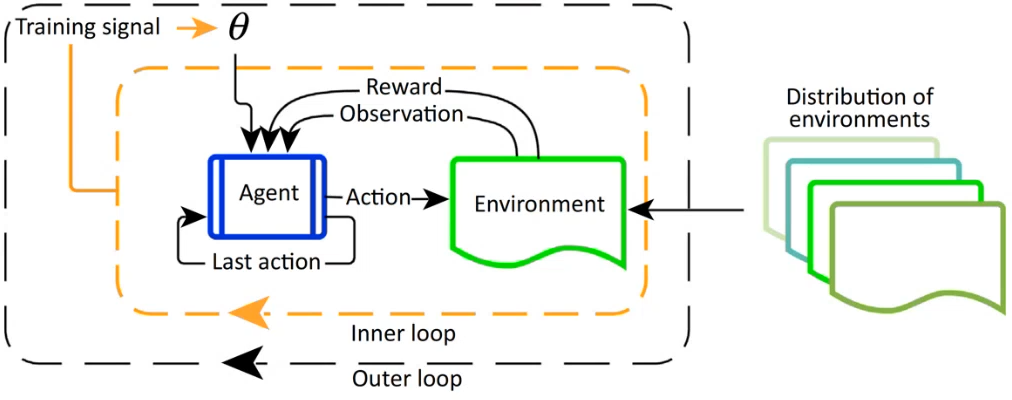
\includegraphics[width=0.6\linewidth]{./img/meta_rl.png}
        \end{figure}
\end{description}

\begin{remark}
    Meta-learning emerges spontaneously from two basic conditions:
    \begin{itemize}
        \item A learning system with some form of short-term memory.
        \item A training environment that exposes the learning system to interrelated tasks.
    \end{itemize}
    If the two conditions are satisfied, the system slowly learns to use the short-term system as a basis for fast learning.
\end{remark}

\begin{casestudy}[RNN meta-learning \cite{rnn_meta}]
    A recurrent neural network is trained on a series of interrelated RL tasks (choose between two slot machines, i.e. bandit problem) varying only on their parametrization. The network interacts with one bandit problem (consisting of two slots) at a time for a fixed number of steps before moving to another one.

    Results show that the agent learns to balance exploration and exploitation: for harder instances (i.e. similar probability of winning) it explores more while easier instances are exploited more.

    Moreover, after some training, the network with its weights fixed is able to explore new bandit problems.

    \begin{figure}[H]
        \centering
        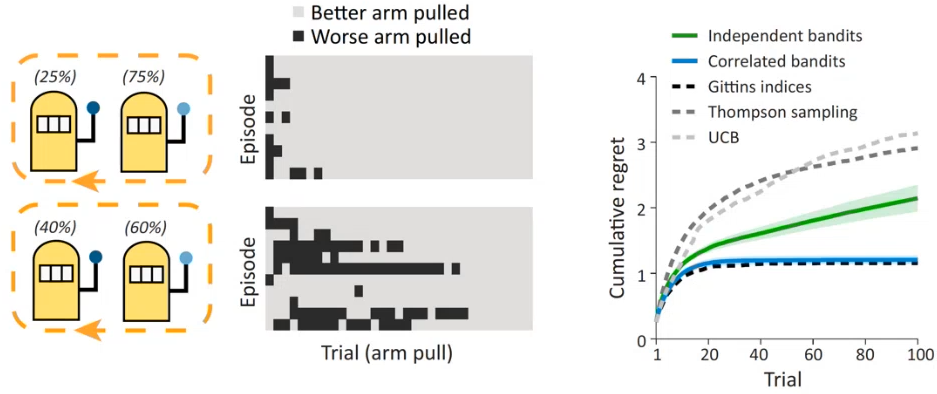
\includegraphics[width=0.6\linewidth]{./img/rnn_meta1.png}
    \end{figure}
\end{casestudy}

\begin{casestudy}[Meta-learning neuronal mapping \cite{meta_cortex}]
    \phantom{}\\
    \begin{minipage}{0.7\linewidth}
        Researchers hypothesized that meta-learning involves the prefrontal cortex where the inner-loop resides.
        On the other hand, dopamine acts as the outer-loop and is responsible for tuning the inner-loop.
    
        Machine simulations are in favor of this hypothesis.
    \end{minipage}
    \begin{minipage}{0.2\linewidth}
        \centering
        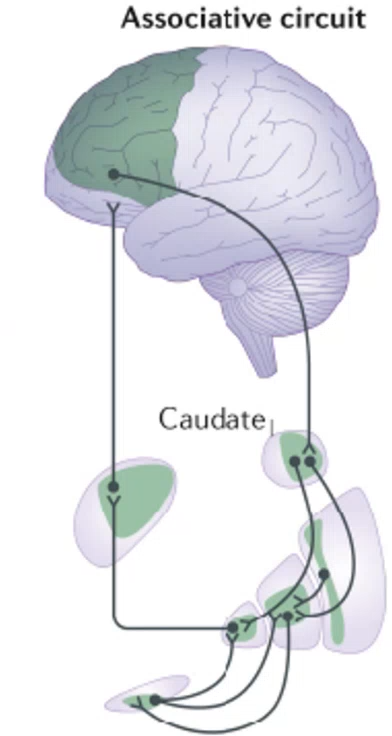
\includegraphics[width=0.7\linewidth]{./img/meta_learning_mapping.png}
    \end{minipage}
\end{casestudy}

